\documentclass[11.5pt]{sig-alternate}
\usepackage[defaultlines=3,all]{nowidow}
\usepackage{hyperref}
\usepackage{tabularx}
\usepackage{graphicx}
\usepackage{blindtext}
\usepackage[utf8]{inputenc}
\usepackage[english]{babel}
\usepackage{lastpage}
\usepackage{float}
\usepackage{comment}
\usepackage{multicol}
\usepackage{dirtytalk}
\usepackage{xcolor}
\usepackage{hanging}
\usepackage{array,url,kantlipsum}
\usepackage{wrapfig}
\usepackage[backend=biber, style=apa]{biblatex}
\addbibresource{notation.bib}
\usepackage{authblk}
\usepackage{caption}
\usepackage{graphicx,subfigure}
\usepackage{authblk}
\usepackage{enumitem}
\usepackage[utf8]{inputenc}
\usepackage{cuted}
\usepackage{fancyhdr}
\usepackage{multirow}
\pagestyle{fancy}
\usepackage{lipsum}
\renewcommand{\headrulewidth}{0pt}
\renewcommand{\footrulewidth}{0pt}
\setlength\headheight{80.0pt}
\addtolength{\textheight}{-80.0pt}
\chead{%
  \ifcase\value{page}
  % empty test for page = 0
 \or 
\includegraphics[width=\textwidth]{headerImage.png}% page=1
  \or 
\includegraphics[width=\textwidth]{headerImage.png}% page = 2
  \or 
\includegraphics[width=\textwidth]{headerImage.png}% page = 3
  \or 
\includegraphics[width=\textwidth]{headerImage.png}% page = 4
  \or 
\includegraphics[width=\textwidth]{headerImage.png}% page = 5
  \else
  
\includegraphics[width=\textwidth]{headerImage.png}
  \fi
}

%\chead{
\includegraphics[width=\textwidth]{headerImage.png}}
\fancyfoot[LE,LO]{Teaching Science to Students with Disabilities Using Socio-Scientific Issues\\           
DOI: 10.14448/jsesd.}
\fancyfoot[CE,CO]{{ }}
\fancyfoot[RE,RO]{\thepage}
\pagenumbering{arabic}
\hypersetup{
    colorlinks=true,
    urlcolor=blue
}
 
\let\oldabstract\abstract
\let\oldendabstract\endabstract
\makeatletter
\renewenvironment{abstract}
{\renewenvironment{quotation}%
               {\list{}{\addtolength{\leftmargin}{1em} % change this value to add or remove length to the the default
                        \listparindent 1.5em%
                        \itemindent    \listparindent%
                        \rightmargin   \leftmargin%
                        \parsep        \z@ \@plus\p@}%
                \item\relax}%
               {\endlist}%
\oldabstract}
{\oldendabstract}
\makeatother

% Left align captions
\captionsetup{justification   = raggedright,
              singlelinecheck = false}


\begin{document}

\title{Teaching Science to Students with Disabilities \\Using Socio-Scientific Issues}

\author[1]{\large \color{blue} Rachel Juergensen}
\author[2]{\large \color{blue} Laura Zangori}
\author[2]{\large \color{blue} Pat Friedrichsen}
\author[3]{\large \color{blue} Troy D. Sadler}



\affil[1]{Delaware State University}
\affil[2]{University of Missouri}
\affil[3]{University of North Carolina at Chapel Hill}
\toappear{}

\maketitle
\begin{@twocolumnfalse} 
\begin{abstract}
\item 
\begin{large}
 \textit{Students with disabilities experience inequitable learning opportunities in science class-rooms. To create equitable learning environments, science teachers must embed supports within their curriculum units. Teachers rely on their beliefs about the capabilities of their students, their role as science teachers, and the goals of science education to adapt their curriculum units. Curricular changes occur through their pedagogical design capacity (PDC) during lesson planning and enactments, in which their beliefs inform their PDC choices. Yet there is little research regarding science teachers’ beliefs about teaching students with disabilities and how they enact their science curriculum materials in general education science classrooms. This qualitative case study focused on one secondary biology teacher who taught a socio-scientific issues (SSI) based unit in a remedial biology classroom. Teacher beliefs and PDC served as the theoretical and analytical frameworks. Data included classroom observations and stimulated recall interviews. Findings show the teacher’s beliefs about her students’ capabilities, role as their science teacher, and goals for science learning drove her PDC. She scaffolded, adapted, and improvised to support learners, while not changing the rigor of the curriculum unit. This study illustrates a vision of equitable science instruction with implications for bringing this vision to life for students with disabilities in science classrooms.}\\
 

   
     
     Keywords: Science, Socio-Scientific Issues, Students with Disabilities
 \end{large}     
\end{abstract}
\end{@twocolumnfalse}

%% ABSTRACT


%% AUTHOR INFORMATION

\textbf{*Corresponding Author, Rachel Juergensen}\\
\href{mailto:rjuergensen@desu.edu}{(rjuergensen@desu.edu)} \\
\textit{Submitted Feb 28, 2023}\\
\textit{Accepted Jun 22, 2023} \\
\textit{Published Online } \\
\textit{DOI: 10.14448/jsesd.} \\

\pagebreak
\pagebreak

\vspace{5mm}
\section*{\vspace{140mm}}
\section*{Teaching Science to Students with Disabilities Using Socio-Scientific Issues}
\begin{large}
Science education reform efforts have long sought to make science relevant to \textit{all} students’ everyday lives and prepare \textit{all} students for responsible citizenship, including diverse learners (Yerrick, 2000). Diverse learners are identified based on: (a) socioeconomic status, (b) race or ethnicity, (c) disability status, and (d) English proficiency (ESSA, 2015; NGSS Lead States, 2013). We focus specifically on students with disabilities, which represents over seven million current K-12 students in the United States (U.S. Department of Education, 2019) and students experiencing difficulty. Many students, not just students with disabilities, experience difficulty learning science (Morgan et al., 2016). Despite this large population of students, there has been little work exploring how to make science accessible to students with disabilities and students experiencing difficulty (Kahn \& Lewis, 2014; McGinnis \& Kahn, 2014; Therrien et al., 2011; Villanueva et al., 2012; Yerrick et al., 2011).

This is a critical area, as all students need access to learn science and develop scientific literacy. Roberts (2007) defines scientific literacy through two distinct, yet interrelated goals, called Vision I and Vision II. Vision I highlights academic knowledge and practices associated with the discipline of science. Vision II asks students to go beyond the content knowledge and practices of scientific disciplines to become informed citizens using their science knowledge to grapple with real-world problems that are complex and include social, economic, and political factors. Socio-scientific issues (SSI) based instruction is unique in its approach as it fulfills both Visions, as science content is situated in global and local issues that connect to students’ lived experiences (Evagorou et al., 2020). Literature bases have emerged showing that SSI improves student learning, interest, and supports development of scientific literacy (Friedrichsen et al., 2021; Dori et al., 2003; Zohar \& Dori, 2003). Yet there is little evidence that SSI teaching has been enacted widely in settings where students with disabilities and students experiencing difficulty are receiving science instruction. As a result, most of what we know about SSI teaching and learning is based on research that does not specifically focus on how SSI teaching can be effectively enacted for this population of students (e.g., Sadler, 2022).

A teachers’ beliefs about how their students can engage with science content, such as through SSI, shapes how they create their classroom environment and enact their curriculum (Bryan, 2012; Remillard, 2005). With this in mind, the goal of this study is to explore an experienced biology teachers’ beliefs about her students in a secondary science classroom serving students with disabilities and students experiencing difficulty and how those beliefs shaped her curricular enactment of an SSI science unit on homeostasis. Our research questions guiding this case study are:

\begin{enumerate}
    \item How do a science teacher’s beliefs about her students with disabilities and students experiencing difficulty inform her enactment of an SSI unit in a secondary general education remedial biology classroom?
    \item How does a science teacher’s role in teaching science to students with disabilities and students experiencing difficulty inform her enactment of an SSI unit in a secondary general education remedial biology classroom?
    \item How does a science teacher’s goal for teaching science to students with disabilities and students experiencing difficulty inform her enactment of an SSI unit in a secondary general education remedial biology classroom?
    \item How does a science teacher plan for an enact an SSI unit for students with disabilities and students experiencing difficulty?
\end{enumerate}

\section*{Theoretical Framework}
\subsection*{Teacher Beliefs and \\Pedagogical Design Capacity}

Teacher beliefs play a critical role in shaping teaching practices (Bryan, 2012; Buehl \& Beck, 2015). However, teacher beliefs have been described as a messy construct due to the use of varying definitions (Pajares, 1992). Philipp (2007) brings clarity to teacher beliefs with the following definition: “Psychologically held understandings, premises, or propositions about the world that are thought to be true” (p. 259). He elaborates that beliefs, in comparison to attitudes, are more cognitive and resistant to chan-ge. Beliefs exist in complex clusters, or belief systems, and play an overriding role in shaping practice (Meis Friedrichsen \& Dana, 2005).

Remillard (2005) defines curriculum materials as “the resources and guides used by teachers” (p. 213). These materials serve as a cornerstone of teaching because teachers use them daily for making decisions about what content to teach and how to teach it (Ball \& Cohen, 1996). Curriculum materials exist in three forms: the curriculum materials as written (formal curriculum), teachers’ lesson planning with the curriculum materials (intended curriculum), and the actual curriculum materials implemented in the classroom (enacted curriculum). Here, we focus on both the intended and enacted curriculum as this provides a means to explore the interactions between teachers’ beliefs and how their beliefs shape curricular enactments (Figure 1; Bryan, 2012). We do this through exploring a teacher’s pedagogical design capacity, or PDC (Brown, 2009). PDC was developed as a theoretical frame for exploring the interplay between mathematics teachers and curriculum materials (Remillard, 2005; Stein et al., 2007). However, this framework has also been used within science education to explore how teachers use their PDC and how educative curricula might further develop the teacher-curriculum relationship (e.g., Davis et al., 2011; Forbes \& Davis, 2010; Knight-Bardsley \& McNeill, 2016). PDC comes into view through observing and analyzing \textit{how} the curriculum is enacted in the classroom. Teachers shape their curricular enactments through offloading, adapting, or improvising (Brown, 2009).

\subsection*{Figure 1}

\begin{figure}[htp]
    \centering
    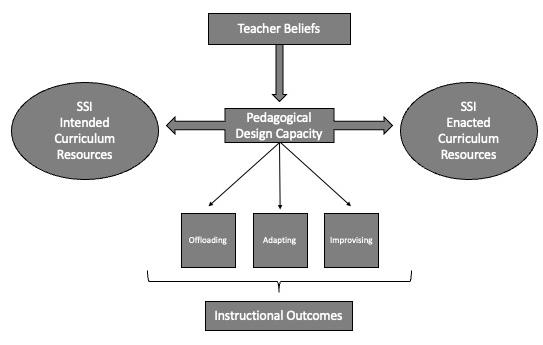
\includegraphics[width=8cm]{figure1.jpg}
 \caption*{Interaction between teacher beliefs and PDC (Adapted from Brown, 2009 \& Remillard, 2005)}
    \label{Interaction between teacher beliefs and PDC (Adapted from Brown, 2009 & Remillard, 2005)}
\end{figure}

When teachers offload their curriculum, they choose to use their curriculum materials as is, following the educational activities and pedagogical moves within the materials closely. When they adapt their materials, they may keep elements but also draw upon their own personal resources to make modifications such as supplementing and/or deleting aspects of the curriculum and may choose to replace the deletion, to substitute with a different resource, or use something they think is better suited to the learning goals. A teacher may also improvise during their curriculum enactment in which they decide “on the fly” to omit, supplement, or adapt materials they had planned to enact. Offloading, adapting, and improvising may all occur within the same lesson, or only one or two of these pedagogical design decisions may be made within a lesson. Ultimately, instructional outcomes result from the ways in which the curriculum is intended and enacted as determined by the teachers’ PDC (Remillard, 2005; Smith et al., 2018).

Each teacher has an individualized relationship with their curriculum resources dependent on various factors which include their knowledge, beliefs, identity, and orientation related to science teaching and prior knowledge about how best to promote science learning (Davis, Janssen, \& Van Driel, 2016). Of these factors, Bryan (2012) states, “teachers’ beliefs mediate the curriculum implementation process” (p. 483) suggesting that beliefs shape teachers’ relationships with curriculum. The framework and the interaction between teacher beliefs and their PDC can help illustrate why the same lesson or unit may be implemented differently depending on the teacher.

\section*{Background Literature}
\subsection*{Teaching Students with Disabilities and SSI}

The biology class that is the focus of this study is referred to as remedial; however, in some science education literature, this type of class in which the student population has been identified as having a disability or experiencing difficulty, has also been called “lower track" (e.g., Yerrick, 2000). Students in these classrooms hold high expectations for their teachers—stud-ents expect their teachers to be able to help them engage with class materials in motivating ways and make content relevant to their lives (Yerrick et al., 2011). In contrast, science teachers tend to perceive these students as having lower abilities, have lowered academic expectations, and focus on simplifying the material through lecture and worksheets (Dori et al., 2003; Yerrick, 2000; Yerrick et al., 2011).

Yet, this method of perceived simplified instruction makes it more difficult for students in remedial classrooms to learn (Scruggs et al., 1993) particularly to learn in the way intended by the NGSS which is more rigorous than past science standards (NGSS Lead States, 2013). Best practices for science lessons in classrooms where students with disabilities and students experiencing difficulty receive science instruction are inquiry-based with proper supports such as peer-to-peer discussions, explicit connections to broad science concepts, tiered materials based on individualized levels of need, vocabulary instruction using multi-modal approaches, critical components of explicit instruction, and giving students problems to consider that require development of critical thinking skills (Brigham et al., 2011; McGrath \& Hughes, 2018; Therrien et al., 2017). Instruction should also be differentiated and include rich scaffolds (Mastropieri et al., 2006; McGinnis \& Kahn, 2014; Therrien et al., 2011; Villanueva et al., 2012).

While SSI based instruction aligns with many of these best practices given its focus on critical thinking, these same attributes make it a demanding pedagogical practice (Friedrichsen et al., 2021; Day \& Bryce, 2011; Eckborg et al., 2013). SSI lessons incorporate science content and practice standards, present challenging questions, support students in using evidence, ask students to think critically (Sadler, 2022) and can support practices such as argumentation (Purwati \& Prasetyanti, 2019). Knight-Bardsley and McNeill (2016) looked at beliefs science teachers held about argumentation-based science curriculum materials. They found that when the teachers’ beliefs about the practice of argumentation was in congruence with argumen-tation-based instruction, then the teachers offloaded the curriculum materials and implemen-ted argumentation practices as articulated in the materials. In contrast, when teachers’ beliefs did not align with scientific argumentation, they deleted those facets of the curriculum and replaced argumentation opportunities with resources that aligned with their beliefs. When this occurred, the intentions of the curriculum materials regarding the implementation of scientific argumentation in the classroom were lost.

Implementing SSI-based lessons requires that teachers hold beliefs that teaching in this manner is an important aspect of science education, as well as beliefs that their students are capable of grappling with the issue (Dori et al., 2003). For example, teachers who believe that it is their responsibility to help students negotiate the ethical dilemmas posed in SSIs and that their students are capable of grappling with complex issues, find ways to enact SSI-based lessons in their classrooms (Zohar \& Dori, 2003). In these situations, students tend to see the science content as relevant and are motivated to learn. However, teachers who believe that students should receive science instruction only as scientific facts because students are incapable of grappling with complexity choose not to implement SSI-based instruction. In these instances, students may not be able to determine how science knowledge pertains to their everyday lives, thus reducing their motivation to learn science.

\subsection*{Teacher Beliefs and Practice}

The construct of science teaching orientations has been used to describe teacher beliefs (Magnusson et al., 1999). In a review of the science teaching orientation literature, Friedrichsen, Driel, \& Abell (2011) found that teacher beliefs relate to the teacher’s role, how students learn science, and their beliefs about the goals of science education influence their teaching practice. For example, Cronin-Jones (1991) found that when a science teachers’ beliefs about student learning did not align with a pedagogical move (e.g., using group work) within curriculum materials, then the teacher deleted that move and replaced it with pedagogical move (e.g., drill and practice) that she believed did impact student learning. While the Cronin-Jones example finds congruence between the teachers’ beliefs and practices, other studies find incongruences between belief and practices \\(Bryan, 2012).

Incongruences between teacher beliefs and practice are visible in studies that focus on students with disabilities. Robinson (2002) found that teachers’ beliefs aligned with supporting their students with disabilities but made “few adaptations” (p. 16) to their materials to support their students with disabilities. Maeng and Bell (2015) found that secondary science teachers modified their curriculum materials to include differentiated instruction yet had varying levels of proficiency and success in implementation. These incongruences between beliefs and practices regarding differentiation may be due to a lack of teacher experience in implementing differentiated instruction (Kimmel et al., 1999). The less experience teachers have in classrooms with students of varying needs, then they may believe themselves inadequately prepared to implement adaptations to their lessons (DeSimone \& Parmar, 2006). Overall, there is a small literature base investigating the alignment of beliefs and practice with experienced teachers (e.g., Bryan, 2012; Buehl \& Beck, 2015) and an even smaller literature base on what this alignment looks like in a remedial science classroom.

\subsection*{Teacher Beliefs and PDC}

Few studies specifically investigate the relationship between teacher beliefs and PDC (Davis et al., 2011; Knight-Bardsley \& McNeill, 2016; Smith et al., 2018). Davis and colleagues (2011) found that teachers use their PDC to align curriculum materials with their beliefs about science learning goals and how those goals aligned with their perceived abilities of their students. When the curriculum materials aligned with teachers’ learning goals and students’ abilities, then they offloaded the curriculum materials and added scaffolds to further support students’ engagement with the materials (Davis et al., 2011). However, when the teachers’ beliefs regarding their students’ abilities conflicted with the curriculum materials, then the teacher chose to delete portions of the curriculum materials and replaced them with other resources that better aligned with learning goals and perceived student abilities (Smith et al., 2018). We did not find instances of investigating teacher beliefs and how beliefs come into play through their PDC of science curriculum materials in secondary remedial science classrooms.

\section*{Methodology}

This was a naturalistic inquiry (Lincoln \& Guba, 1985) that sought to describe and interpret how an experienced general education high school biology teacher, Ms. Sting (pseudonym), enacted an SSI unit within her remedial biology classroom. We used a descriptive single case study method (Yin, 2017) as our goal was an in-depth analysis to explore how this biology teachers’ beliefs about her students, her role in the classroom, and her goals for teaching science informed her planning and enactment of an SSI unit. With how questions, the case study method provides space for in-depth study and “detailed probing” (Lincoln \& Guba, 1985, p. 358) in a real-life setting to gather sufficient information to understand the teacher, the context, and the system in which the case takes place to acquire an in-depth understanding of the phenomenon
(Yin, 2017).

\subsection*{Study Context}

\textbf{Participant Selection.} Our research team has worked with a professional learning community (PLC) of biology instructors at a secondary \\school within a small Midwestern city for over five years (Friedrichsen et al., 2021). Ms. Sting was a member of this PLC. In the school district in which this study takes place, students are either enrolled in honors, general, or remedial biology sections. All students enrolled in the remedial biology section were either identified as having a disability or were identified as students who experienced difficulty (academically or behaviorally). Students not identified as having a disability or experiencing difficulty were not enrolled in the remedial section of biology.

The PLC participated in a five-day summer professional development (PD) workshop to design a new SSI unit. The daily PD schedule, information about the larger project, and data from the larger study in which the PD was situated is detailed in Friedrichsen et al. (2021). The PD centered on the SSI Teaching and Learning framework (Sadler, Foulk, \& Friedrichsen, 2017). During the PD, the PLC worked with instructional tools designed to support implementation of SSI teaching and learning: (1) a 2D Diagrammatic Modeling tool to support students in developing and using models of their own design to make sense of phenomenon within the unit, and (2) a graphic organizer called the Star Chart to support students in looking at different dimensions of the issue.

We chose Ms. Sting for an in-depth analysis because her case study provided a particularly clear, concise, and vivid example of an experienced secondary science teacher enacting an SSI unit in a general education classroom serving students with disabilities and students experiencing difficulty. Ms. Sting taught biology for over 20 years and had spent the previous three years teaching this population of students in remedial biology classrooms. During the semester this data was collected, there was no special education co-teacher in the classroom, so Ms. Sting made curriculum enactment decisions on her own. Therefore, her PDC was evident as she interacted with the unit materials to design instruction and taught the unit to students with disabilities and students experiencing difficulty within her classroom.

\textbf{Curricular Context.} All students in this state take high school biology, and biology is the only science subject with a mandated exam that students must pass to graduate. Most students take biology in their sophomore year and are either enrolled in an honors, general, or remedial section. The school used a block schedule, so the class met every other day for 90 minutes.

Ms. Sting taught the SSI unit written during the workshop, called the Vaping Unit. The focal issue of the Vaping Unit was whether e-cigarettes should be regulated to protect public health. See Friedrichsen et al. (2021) for the full unit. At the start of the unit, students read news releases on the prevalence of vaping and shared ideas about the regulation of vaping. Next, they drew initial models predicting the effects that vaping has on body systems. From there, students learned about homeostasis, feedback loops in body systems, macromole-cules, cell transport and membranes, and what happens when there is a disruption in homeostasis at the molecular level. Throughout each lesson, students re-visited the vaping issue to consider regulation. The unit was NGSS-aligned with explicit foci on scientific practices of modeling and argumentation as well as crosscutting concepts of systems, system models, and stability and change. The unit ended with students creating a final model and a culminating project, both of which served as summative assessments. For the model, students were given the following prompt: \textit{“Your friend has been vaping nicotine containing e-cigarettes for a while now. When she first started vaping, she had more energy, a smaller appetite, and more focus, and she generally felt happier. Now that she has vaped these nicotine containing e-cigarettes for a while, she realizes that she feels tired, irritable and unfocused if she doesn’t vape about the same amount every day. She also finds that if she vapes higher amounts of nicotine than normal, she feels her heart beat faster and starts to sweat. Draw a model to explain what is occurring within your friend’s body systems that requires her to have the same amount of nicotine in the e-cigarette to feel normal.”} For the culminating project, students created a poster, infographic, or wrote a newspaper article taking a position on vaping regulations. In their culminating projects, they considered the consequences of the regulations for all stakeholders, such as teen consumers, tobacco farmers, and small business owners.

\subsection*{Data Collection}

As suggested by Yin (2017), our data collection included observational data, interviews, and a questionnaire to elicit Ms. Sting’s professed beliefs.

\textbf{Observations.} The second author observed and took field notes of Ms. Sting’s entire unit enactment (11 class periods) from October through February in one remedial biology course section with 15 students. Field notes captured the physical setting, the social environment of the classroom including verbal and non-verbal communication between the teacher and students, and the implementation of the curriculum materials as well as any changes to the curriculum materials (Patton, 2002).

\textbf{Interviews and Questionnaire.} The authors designed interview questions based on the theoretical framework including teacher belief categories identified in Friedrichsen, Driel, \& Abell (2011) and PDC as described by Brown (2009). We designed the questions to elicit how Ms. Sting viewed her role in a remedial classroom, how students learn science, the goals of science education for students with disabilities and students experiencing difficulty, and what she considered when she planned curriculum enactment. The first interview was a focus group including all PLC members led by the third author and lasted 45 minutes. Next, the second author interviewed Ms. Sting eleven times immediately after each lesson for 5 – 15 minutes with questions that focused on the lesson just taught. At the conclusion of the unit, the second author conducted a 45-minute interview with Ms. Sting. Ms. Sting completed a follow-up questionnaire designed to further elicit her beliefs about teaching the vaping unit in a secondary remedial biology classroom.

\subsection*{Data Analysis}

Data analysis was conducted by all authors in weekly meetings for iterative analysis. The authors began analysis with the theoretical framework of teachers’ beliefs (Friedrichsen, Driel, \& Abell, 2011) and PDC (Brown, 2009). Using classical content analysis (Patton, 2002), we read through the data corpus in chronological order to look for patterns to identify Ms. Sting’s core consistencies, meanings about beliefs, and PDC. At each meeting, we re-evaluated emerging patterns about Ms. Sting’s beliefs and PDC, debated interpretations, and conduc-ted negative case analyses (Lincoln \& Guba, 1985). From these discussions, we documented Ms. Sting’s consistent and frequent reference to three themes across the data in which she discussed or demonstrated her perspectives on 1) the standards she held for her students, 2) the role of supports, and 3) connections between science content and her students’ lives. These themes were the basis for the three main beliefs we identified that Ms. Sting held connected to our first three research questions.

To answer our fourth research question, we que-ried all data that were coded for one of the three belief themes for the first three research questions (i.e., students’ capabilities, the role of supports, and connections between science content and her students’ lives). We then used the theoretical framework as an analytical framework and analyzed these data using a priori codes from PDC (Brown, 2009; offloading, adapting, and improvising) to look for how Ms. Stings’ beliefs shaped her use of the SSI materials. From this analysis, we were able to refine our codes to answer our fourth research question as offloading with scaffolding (teaching the curriculum as is but spending time to carefully support students during the lesson), adapting through insertion (adapting the curriculum to add to the materials), and improvising (decisions made in the teaching moment in which Ms. Sting adds to the materials or modifies existing materials in response to her students’ needs). When analysis was complete, we did peer debriefing (Lincoln \& Guba, 1985) with an experienced researcher who was not involved in the original data analysis to check for the credibility and confirmability of the results. We also sent our themes and evidence from the data corpus to Ms. Sting for member-checking. In both cases (peer debriefing and member checking), our articulations of beliefs and evidentiary support for those inferences were supported.

\textbf{Trustworthiness.} For this work, we used a variety of strategies to build trustworthiness (Lincoln \& Guba, 1985). We had prolonged engagement with the participant over a 3-month period, completed live observations for each lesson, and collected multiple sources of data for triangulation. The authors met weekly over an eight-month period for extended periods of iterative analysis cycles. In each meeting, we re-evaluated data and coding, debated interpretations, and completed negative case analysis. Finally, we completed member checking with the participant in which we sent them our interpretations, and she agreed with our conclusions.

\section*{Findings}

Using the interaction between teacher beliefs and PDC as both a theoretical and analytical framework provided insight into the way Ms. Sting’s beliefs about her students, her role, and her goals for teaching science informed her enactment of an SSI unit for students with disabilities and students experiencing difficulty in her secondary general education remedial biology classroom. Several interesting findings emerged illustrating these interactions. Next, assertions will be described for each of the research questions.

\textit{RQ1: How do a science teacher’s beliefs about her students with disabilities and students experiencing difficulty in science inform her enactment of an SSI unit in a secondary general education remedial biology classroom?}

Assertion: \textbf{Ms. Sting believed the same curriculum benchmarks should be used in her remedial science classroom as in all other biology sections.} Ms. Sting was explicit that her students would engage in the same curriculum and do as well in the unit as the other biology sections. She articulated these expectations with her students “We had to show growth [to school administration] and we were up front with the kids about that, that, you know, our goal here is to show growth and we want you to grow…” (Final Interview). Ms. Sting’s expectation was that her students would participate in the lessons and complete the culminating project and final models so that their growth across the unit was evident to her as well as to school administrators. She was explicit with these expectations with her students in which she reiterated what she said to her students: “We expect that when we get to that assessment that you guys [students] are going to do as well, or nearly as well, as the other classes [general and honors]” (Final Interview). She was clear in her expectations that her students would complete and submit culminating projects and final models that were comparable to those completed in the other biology sections.

She recognized that the SSI unit gave the students opportunities to use their scientific knowledge to create and defend a position on a contentious issue. Because the students were required to use their scientific knowledge to think critically, she stressed that the curriculum sho-uld be presented to her students as intended so they would be prepared to debate the vaping issue: “I believe…that all students can be taught and think critically in science” (Questionnaire). She stressed that implementing the curriculum as intended was critical for her students’ critical thinking development. Yet Ms. Sting’s beliefs also included the recognition that the SSI curriculum materials would be challenging because, as she stated to us, her students were frequently not asked to show and synthesize knowledge and think critically in their prior classes. To her, an important part of the time and support required for the implementation was through the instructional tools (modeling tool and Star Chart) because these tools would give her students opportunities to make their thinking visible and use their critical thinking skills.

When Ms. Sting was asked how she thought the instructional tools would support student learning in her remedial biology sections, she articulated that “they [the students] can do this!” (Final Interview). Ms. Sting was explicit with us, and with her PLC, in her beliefs that her students could meet the challenges posed within the SSI unit. During the focus group interview with the rest of her PLC, she commented on the importance of giving students in her classes these opportunities: “you might even see the [remedial] kids who think, you know, if you put that stretch question on a test or as a challenge, I mean, like, they might surprise you” (Focus group interview). Overall, Ms. Sting believed her students were capable of meeting the curriculum benchmarks. In addition, she wanted her students, as well as other teachers and administrators, to also see they were able to meet these benchmarks.

\textit{RQ2: How does a science teacher’s role in teaching science to students with disabilities and students experiencing difficulty inform her enactment of an SSI unit in a secondary general education remedial biology classroom?}

Assertion: \textbf{Ms. Sting’s articulated beliefs focused on the expectations of her students to meet the benchmarks of the curriculum materials and she considered that her role was to ensure the materials included appropriate supports to “level the playing field” so her students could meet the benchmarks.} Ms. Sting reviewed the PLC’s planned SSI curriculum and thought about her students’ strengths and areas for growth and put supports in place to meet them at their current levels:

\begin{quote}
    My role basically was to take what they [the other biology teachers] did and make it work in the [remedial] classroom so that meant I had to change, maybe how I did the notes or change maybe how I was going to do the lab... or I would find an alternative activity that we liked that was more active or hands-on that would get the same result. So, I would take that information and then make it work (Interview)
\end{quote}

As evident in this quote, Ms. Sting found it important to differentiate instruction for her students. She also stated: “I would say that you can’t do it [teach in a remedial classroom] effectively if you don’t differentiate your instruction. The whole point of that is to meet the kids where they are and scaffold them up” (Interview). She talked about differentiation methods she regularly used in her instruction. For example, for assignments that involved reading, she provided the same reading at different reading levels and provided graphic organizers to support
notetaking as students read. She also talked about differentiation and scaffolding specific to the Vaping Unit: for the Star Chart activity, she differentiated by using different colors to represent different areas for students to research so students could easily tell which point on the chart was their responsibility (Interview). She also talked about scaffolding her students’ modeling practices by providing a set of symbols that could be used as a starting place for the modeling activities (Interview). At the conclusion of the SSI unit Ms. Sting reflected on her students’ success with the unit: “You know, you couldn’t tell the difference between our kids and the honors kids when you looked at those [culminating projects and final models], they were that great” (Interview). Ms. Sting articulated this point several times - that the culminating projects and final models completed by her students were as strong as those produced in the other biology sections. She attributed this to the supports she put in place that “leveled the playing field” and helped her students meet the benchmarks of the curriculum materials.

\textit{RQ3: How does a science teacher’s goal for teaching science to students with disabilities and students experiencing difficulty inform her enactment of an SSI unit in a secondary general education remedial biology classroom?}

Assertion: \textbf{Ms. Sting believed the goal of teaching science to students with disabilities and students experiencing difficulty was to make explicit connections between the relevance of the science content to the lives of her students.} Ms. Sting enacted her goal of delivering instruction that her students would view as relevant to their lives, and the Vaping Unit aligned with her beliefs. Within her lessons she tried to make explicit connections between what was happening in biology and her students’ lives stating:

\begin{quote}
    I think our whole goal was, yeah, we had to get them ready for the [mandated final] exam\dots but that was almost peripheral, because we like, we have to make this [content] relevant so that they know that actually this is about them as a biological organism, you know, they’re going to need these principles. (Interview).
\end{quote}

As evidenced within this quote, Ms. Sting’s focus was not on how well students did on standardized tests, but how they understood the relationship of the focal issue to their lives. She articulated that while the relevance of the biological content was explicit to her students' experiences within the SSI unit, this was something she had to build into her other biology units. She was explicit that this was her overarching goal of biology instruction - to make all the curriculum relevant to students’ lives so they could see and make connections between biology and themselves. She articulated that this belief was not only important for students’ critical thinking, but it was also a key to getting students to engage with the materials because it provided a “…modality that empowers them to want to learn” (Questionnaire). She identified that the vaping issue central to the SSI materials was so relevant to their lives, it was imperative that she include all aspects of the issue and the instructional tools central to the issue to her implementation.

\textbf{Summary.} Our findings indicate that Ms. Sting held beliefs that she needed to hold high expectations for her students. Within the discussion of her beliefs, we found that she had an expectation that her students could be as successful as those students in honors and general biology classrooms. Her beliefs included the criticality of support through differentiation and scaffolding so her students would be successful, and their successes evident to themselves as well as to others. In addition, for students to see the relevance of learning the material, then the curriculum materials should make explicit connections between the content and their lives.

\textit{RQ4: How does a science teacher plan for and enact an SSI unit for students with disabilities and students experiencing difficulty?}

Assertion: \textbf{Ms. Sting took her students’ academic and behavioral needs into careful consideration when enacting the unit and scaffolded, adapted, and improvised the curriculum so they could be successful.} Ms. Sting used information she gathered from her students and their classroom performance to make instructional adjustments necessary before, during, and after lessons. Ms. Sting’s most frequent modification to the Vaping Unit was offloading with scaffolds. She taught the intended SSI unit (offloading) but also spent time providing extra support. Throughout the unit, Ms. Sting maintained a word wall (Figure 2; not included in the honors or general classes) that included a drawing depicting each homeostasis vocabulary word. The word wall provided students with a constant visual reference for new vocabulary throughout the unit, and Ms. Sting consistently referenced it when new terms emerged: “We are going to take the idea of maintaining a constant internal environment and then talk about feedback loops. [Points out homeostasis on word wall.]” (Field Notes). Students were observed frequently using the word wall as they were working on readings and assignments during the Vaping Unit.

\subsection*{Figure 2}

\begin{figure}[htp]
    \centering
    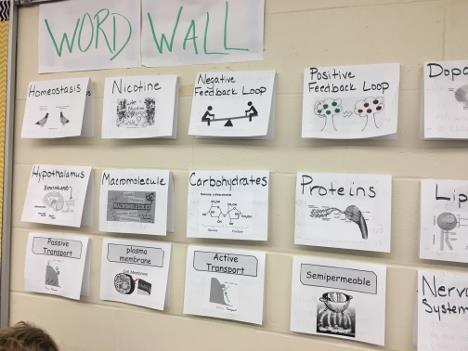
\includegraphics[width=8cm]{figure2.jpg}
 \caption*{Word Wall}
    \label{Word Wall}
\end{figure}

Ms. Sting provided students with a checklist for the models they developed throughout the unit so they would be able to check for important elements in their own models (Field Notes). She explained, “I felt scaffolding in a list for them -my model has this, check, my model has this, and then they get to decide how to obviously show and explain that” (Interview). The unit called for students to work individually on all five points of the Star Chart. Ms. Sting adapted this instructional tool by placing students in small groups and assigning one star point to each small group (in addition to color coding discussed above). As each group reported what they found for their point, she recorded their findings on the Smartboard so all student groups could add the information to their Star Chart (Field Notes).

Overall, the use of scaffolds was evident throughout her implementation of the Vaping Unit, and Ms. Sting acknowledged this: “There is a lot of scaffolding going on. Yeah…you just have to kind of step back and build the pieces up” (Focus group interview). Ms. Sting also saw the scaffolds as a way of offering her students choices within her lessons. For example, when students were modeling feedback loops, a student asked if she wanted them to make a flow chart and Ms. Sting responded that the students could do it in whatever way made the most sense to them (Field Notes). She stated, “The other important aspect that makes [remedial classrooms] successful is that once you have buy-in on an idea like the Vaping Unit and kids have the freedom to learn in the way that suits them best, you will end up with amazing results” (Questionnaire). After Ms. Sting offered scaffolds, her students had the choice whether to continue using the scaffolds or choose different methods of support that she provided.

The second most frequently used strategy was adapting the curriculum, and the changes she made reflected her own personal resources. Her most frequent method of adapting was changing the order of the lesson. For example, a critical component of SSI instruction is the introduction of the issue. While the unit suggested introducing the vaping issue through reading and writing about the issue, Ms. Sting recognized her students were “very interested in talking about” (Interview) the issue with her and with each other. While she did use the reading and the writing assignment with the curriculum unit, she adapted the unit so that this came after a discussion. She introduced the issue by using an anonymous poll in which she told her students “Think about everything we know [about vaping]. I’ll give you a couple of minutes to think about it and then we’ll discuss” (Field Notes). The poll results were displayed on the Smartboard, and results were used to initiate whole class discussions about vaping. Ms. Sting then assigned readings on vaping and placed students in small groups to answer questions about the readings. She indicated that she changed the order because doing so would provide better support for her students through discussing their ideas and then talking through the reading and writing assignment in small groups. She elaborated that she changed the lesson order frequently because she wanted to provide more examples of how something occurs before asking students to explore the idea on their own.

She frequently utilized different student grouping patterns as well as different levels of reading materials within the unit to meet students’ needs, allowing students to choose to work with a group or individually. She used the Newsela website (https://newsela.com/) to choose relevant articles about vaping and employed features on the website to provide the same article at different reading levels (Field Notes). She stated, “And then we split that up into like even three different groups for like low, medium, high reading levels” (Interview) so that all students could participate in the readings and discussions about the readings. Ms. Sting was able to use her own personal resources such as rearranging the order of her instruction or using online resources to help adapt the curriculum for her students.

The third most used strategy was \textit{improvising.} When Ms. Sting noticed her students struggling with elements of the lesson, she would modify in the moment so she could help them be successful. For example, her students asked clarifying questions when confused during a lesson and she would provide additional examples or return to prior concepts for re-teaching (Field Notes). She mentioned a conversation she had with a member of her PLC who was frustrated about his students’ performance: \\“And he thought it’s like, what he did yesterday was totally a waste. He was just like, ‘This was bad.’ And I said, ‘Oh, that happens to me a lot.’ So, I have to back up [revisit the material] and figure it out” (Interview). In another lesson, the students were to model a feedback loop and add arrows to show a sequence of events. When Ms. Sting noticed her students struggling to figure out how to get started, she improvised in the moment to provide more support. She initiated a class discussion asking students what emojis (a familiar form of communication) they could use to show how vaping affected a person. She stated: “We are going to turn this into a flow chart, we are going to add arrows so we can see the sequence of events. If you were picking an emoji, how would you show this?” (Field Notes). Within the SSI unit, developing the models was designated for only a few minutes of class time; however, when Ms. Sting realized students needed extra time with modeling, she extended the modeling activity to take the entire class period. This improvisation was critical to the success of the SSI unit, as the models served as sense-making tools for the connections between vaping and body systems. In expanding the modeling time, she provided students time to think about how they wanted to develop and use their models and she also provided class discussions for students to share ideas on how they could show feedback occurring within different body systems. Ms. Sting’s attention to recognizing and providing her students with extra time for modeling was vital to students’ success.

\textbf{Summary.} Ms. Sting did not omit any of the SSI materials. Instead, her beliefs drove her to adopt the materials as-is and supplement them with scaffolds and differentiation. She scaffolded student experiences with strategies such as a word wall to support student use and understanding of vocabulary and added discussions to help each other think about how they could show their ideas during modeling. Importantly, she viewed these scaffolds as providing more choice and flexibility to the students as they had some autonomy in terms of how they would use these scaffolds. She also adapted lessons by changing the order of her presentation and adding explicit examples. When she improvised, it was to further support her students in the curriculum materials by figuring out how to draw on their everyday experiences to use as the foundations for their inquiry into the science content and SSI.

\section*{Discussion}

A teachers’ beliefs determine her classroom actions (Bryan, 2012; Cronin-Jones, 1991; Knight-Bardsley \& McNeill, 2016; Remillard, 2005; \\Smith et al., 2018). When considering innovative learning activities, like those seen in SSI teaching, many science teachers hold the belief that “some students simply can’t do it” (Zohar \& Dori, 2003, p. 146), but learning data shows otherwise (Dori et al., 2003; Yerrick, 2001; Yerrick et al., 2011). Our intent here was to explore what a general education biology teacher believed about students with disabilities and students experiencing difficulty in her remedial biology classroom and how those beliefs influenced her PDC within the enactment of SSI curriculum materials. SSI-based instruction for students with disabilities and students experiencing difficulty is a little explored area in the literature and there is much to learn about how general education science teachers can effectively use their curriculum materials to teach this population of students in the general education classroom. This becomes even more critical when a Special Education co-teacher is unavailable, and the general education teacher has to rely on their own beliefs and PDC for their curriculum unit implementations, as we observed here.

Overall, we found Ms. Sting’s beliefs about her expectations for her students within an SSI unit and her practice of the SSI unit to be consistent; her beliefs aligned with those necessary to support her enactment of an SSI unit in an inclusive classroom. She did not omit any of the unit and instead found ways to add supports into the unit because she believed that her students were capable learners that needed these opportunities to grapple with complex ill-structured problems and engage in critical thinking. She also viewed the SSI unit as an important aspect of science education because she believed that science content should be presented in ways that are connected to students’ everyday lives. Her beliefs aligned with the fundamental aspects of SSI (ill-structured problems that connection to everyday life and require critical thinking) but, at the same time, are dimensions of teaching not typically included in science instruction for students with disabilities and students experiencing difficulty (Dori et al., 2003; Yerrick, 2000; Yerrick et al., 2011; Zohar et al., 2001). We found that Ms. Sting believed her students were just as capable of engaging with an SSI-based unit as students in the general and honors classes if she included differentiation and scaffolds for them to be successful. She articulated this as “leveling the playing field.”

How Ms. Sting “leveled the playing field” was evidenced within her planning and enactment of the SSI curriculum resources. She used her PDC to differentiate and scaffold the unit, without omitting any of parts or simplifying the unit. Rather, her PDC approach was to adopt the curriculum as is and add to the materials so her students could engage fully with the SSI-based unit. One way she did this was by embedding critical components of explicit instruction into her more inquiry-based SSI instruction as advocated by Therrien and colleagues (2017) to support her students throughout the unit. While she planned ways to support her students, she also made in-the-moment adjustments (her improvisations). These adjustments provided additional unplanned, scaffolded support such as altering her pacing to slow down and provide more time for students to use the instructional tools to make sense of the content. If Ms. Sting had omitted the Star chart and/or eliminated the students’ creation of the 2D diagrammatic models, then the intentions embedded in the curriculum unit would be lost. Ms. Sting’s focus on figuring out how to differentiate, scaffold, and provide additional time for these instructional tools was critical to the implementation, and to the success, of the SSI unit in her classroom.

This in-depth look at Ms. Sting adds to the literature in new and significant ways as it merges and builds on three different literature bases. First, prior work on SSI teaching beliefs focuses on teachers in general, honors, and/or specialty science classrooms and has not included science teachers who plan and deliver instruction to students with disabilities and students experiencing difficulty (Friedrichsen et al., 2021; Day \& Bryce, 2011; Eckborg et al., 2013). Second, prior work on students with disabilities focuses on the scaffolds and differentiation students require for learning gains and offers little attention to how these best practices align with teacher beliefs (Brigham et al., 2011; McGrath \& Hughes, 2018; Therrien et al., 2017). Lastly, literature that focuses on science teachers’ beliefs about students with disabilities and students experiencing difficulty and how those beliefs manifest in their teaching practice is limited and has not included SSI teaching and learning (DeSimone \& Parmar, 2006; Kimmel et al., 1999; Maeng \& Bell, 2015; Robinson, 2002). The examination of Ms. Sting’s beliefs extends across these three literature bases providing the foundation for SSI-based instruction for students with disabilities and students experiencing difficulty.

\section*{Implications}

Our goal was to provide sufficient information so that another researcher can use this study to make their own judgement of transferability to a new case (Lincoln \& Guba, 1985). Similar research in unique classroom contexts serving students with disabilities and students experiencing difficulty would further inform the understanding of teacher enactments of SSI in classrooms that include this population of students. Work exploring teachers’ beliefs must also include their classroom practice, as there is little science education literature that explores the congruence, or incongruence, between beliefs and practice and how teachers’ beliefs inform their PDC (Davis et al., 2011; Knight-Bardsley \& McNeill, 2016; Smith et al., 2018).

This work also informs professional development activities. General education science teachers require time and support in exploring and reflecting upon their beliefs as well as mentoring and coaching for teachers to revise and refine their beliefs about their students’ capabilities for science lessons generally, and specifically SSI-based lessons. Mentoring and coaching should continue into the classroom with opportunities to plan and enact SSI lessons and reflect on their enactments with a professional development coach. Reflection may provide an opportunity for their beliefs to shift regarding the capabilities of their students with disabilities and students experiencing difficulty (Knight-Bardsley \& McNeill, 2016).

In addition, the importance of adding differentiation, scaffolding, and elements of explicit instruction within the design of SSI curriculum materials for use in classrooms where students with disabilities and students experiencing difficulty receive science instruction must be emphasized. As McGinnis and Kahn state, “students with mild disabilities, in particular, are capable of high-level disciplinary engagement with scientific concepts and procedures if they are \textit{supported appropriately}” (McGinnis \& Kahn, 2014, p. 236, emphasis added). Appropriate supports such as teacher responsiveness to pacing, adapting assigned readings to students reading/comprehension level, using inquiry-based approaches with embedded explicit instruction components, and providing multiple representations of abstract concepts are essential to teaching science to students with disabilities and students experiencing difficulties (Brigham et al., 2011; McGrath \& Hughes, 2018; Therrien et al., 2017). Science teachers self-report that they feel underprepared to teach science because they are unsure of how to make meaningful adaptations to their curriculum materials to support students with disabilities (Kahn \& Lewis, 2014). They may require specific strategies and examples of appropriate supports as well as specific rationales for including aspects of the curriculum unit to feel prepared to implement lessons in their science classrooms for this population of students (DeSimone \& Parmar, 2006; Kimmel et al., 1999; Smith et al., 2018). Therefore, SSI units need to include specific ways to appropriately support students in lessons. For example, using educative curriculum material heuristics to design SSI materials would lead to curriculum materials that support teachers in ideas for how they might differentiate and/or suggestions for how to scaffold instruction for their students (e.g., Beyer \& Davis, 2009).

\section*{Conclusion}

Science must be accessible to all students, so they are able to develop scientific literacy and become informed citizens (Roberts, 2007). Classrooms that serve students with disabilities and students experiencing difficulty require teachers who are flexible with their curriculum and instruction to provide students with rich science experiences (McGinnis \& Kahn, 2014). For this to occur, science teachers must believe that science is accessible to all their students, as a teacher’s beliefs about her students influence her practice and vice-versa (Bryan, 2012). These beliefs are realized through the teachers’ PDC, which are the decisions they make about their curriculum enactments (Brown, 2009). These decisions are defined by what learning they expect from their students in the classroom. Our findings indicate that the teacher within this remedial science classroom held and acted on her beliefs which prompted her to figure out ways to provide a similar curriculum unit experience as was provided in the general biology and honors biology classes. She did this through her PDC in which she scaffolded, adapted, and improvised during her unit enactment. In turn, her changes to the curriculum unit implementation supported her students to be successful within the same SSI unit that their peers in honors and general biology received. Ms. Sting is an exemplar for how to think about, support, and teach science to students with disabilities and students experiencing difficulty. This case study illustrates a vision for how to accomplish equitable science instruction with practical implications for bringing this vision to life in a general education science classroom.


\clearpage
\section*{References}\par 

\leftskip 0.25in
\parindent -0.25in 
%%%

Ball, D. L., \& Cohen, D. K. (1996). Reform by the book: What is—or might be—the role of curriculum materials in teacher learning and instructional reform? Educational Researcher, 25(9), 6-14. \\https://doi.org/10.3102/0013189X025009006

Beyer, C., \& Davis, E. A. (2009). Supporting preservice elementary teachers’ critique and adaptation of science lesson plans using educative curriculum materials. Journal of Science Teacher Education, 20(6), 517. https://doi.org/10.1007/s10972-009-9148-5

Brigham, F. J., Scruggs, T. E., \& Mastropieri, M. A. (2011). Science education and students with learning disabilities. Learning Disabilities Research \& Practice, 26(4), 223-232. https://doi.org/10.1111/j.1540-5826.20\\11.00343.x

Brown, M. W. (2009). The teacher-tool relationship. In J. T. Remillard, B. A. Herbel-Eisenmann, \& G. M. Lloyd (Eds.) Mathematics teachers at work: Connecting curriculum materials and classroom instruction (pp. 17-36). Routledge.

Bryan, L. A. (2012). Research on science teacher beliefs. In B. Frasier, K. Tobin \& C. J. McRobbie (Eds), Second international handbook of science education (pp. 477-495). Springer. https://doi.org/10.1007/978-1-40\\20-9041-7\_33

Buehl, M. M. \& Beck, J. S. (2015). The relationship between teachers’ beliefs and practice. In H. Fives \& M. G. Gill (Eds), International Handbook of Research on Teachers’ Beliefs (pp. 66-84). Routledge.

Cronin‐Jones, L. L. (1991). Science teacher beliefs and their influence on curriculum implementation: Two case studies. Journal of Research in Science Teaching, 28(3), 235-250. https://doi.org/10.1002/tea.3660280305

Davis, E. A., Beyer, C., Forbes, C. T., \& Stevens, S. (2011). Understanding pedagogical design capacity through teachers’ narratives. Teaching and Teacher Education, 27(4), 797-810. https://doi.org/10.1016/j.tate.2011.01.\\005

Davis, E. A., Janssen, F. J., \& Van Driel, J. H. (2016). Teachers and science curriculum materials: Where we are and where we need to go. Studies in Science Education, 52(2), 127-160. https://doi.org/10.1080/03057267.\\2016.1161701

Day, S. P., \& Bryce, T. G. K. (2011). Does the discussion of socio-scientific issues require a paradigm shift in science teachers’ thinking? International Journal of Science Education, 33(12), 1675–1702. https://doi.org/10.1080/\\09500693.2010.519804

DeSimone, J. R., \& Parmar, R. S. (2006). Issues and challenges for middle school mathematics teachers in inclusion classrooms. \\School Science and Mathematics, 106(8), 338-348. https://doi.org/10.1111/j.1949-8594.20\\06.tb17754.x

Dori, Y. J., Tal, R. T., \& Tsaushu, M. (2003). Teaching biotechnology through case studies – can we improve higher order thinking skills of nonscience majors? Science Education, 87(6), 767–793. https://doi.org/10.1002/\\sce.10081

Evagorou, M., Nielson, M., \& Dillon, J. (Eds.) (2020). Science teacher education for responsible citizenship. Springer. https://doi.\\org/10.1007/978-3-030-40229-7

Every Student Succeeds Act, 20 U.S.C. § 6301 ([ESSA] 2015). https://www.congress.gov/\\bill/114th-congress/senate-bill/1177

Forbes, C. T., \& Davis, E. A. (2010). Curriculum design for inquiry: Preservice elementary teachers’ mobilization and adaptation of science curriculum materials. Journal of Re-search in Science Teaching, 47(7), 820-839. https://doi.org/10.1002/tea.20379

Friedrichsen, P. J., Ke, L., Sadler, T. D., \& Zangori, L. (2021). Enacting co-designed socio-scientific issues-based curriculum units: A case of secondary science teacher learning. Journal of Science Teacher Education, 32(1), 85-106.

Friedrichsen, P., Driel, J. H. V., \& Abell, S. K. (2011). Taking a closer look at science teaching orientations. Science Education, 95(2), 358-376.

Kahn, S., \& Lewis, A. R. (2014). Survey on teaching science to K-12 students with disabilities: Teacher preparedness and attitudes. Journal of Science Teacher Education, 25(8), 885-910. https://doi.org/10.1007/s10972-014-9406-z

Kimmel, H., Deek, F. P., Farrell, M. L., \& O'Shea, M. (1999). Meeting the needs of diverse student populations: Comprehensive professional development in science, math, and technology for teachers of students with disabilities. School Science and Mathematics, 99(5), 241-249. https://doi.org/10.1111/\\j.1949-8594.1999.tb17482.x

Knight‐Bardsley, A., \& McNeill, K. L. (2016). Teachers’ pedagogical design capacity for scientific argumentation. Science Education, 100(4), 645-672. https://doi.org/10.1002/\\sce.21222

Lincoln, Y. S., \& Guba, E. G. (1985). Naturalistic Inquiry. Sage Publications. https://doi.\\org/10.1016/0147-1767(85)90062-8

Maeng, J. L., \& Bell, R. T. (2015). Differentiating science instruction: Secondary science teachers’ practices. International Journal of Science Education, 37(13), 2065-2090. https://doi.org/10.1080/09500693.2015.106\\4553

Magnusson, S., Krajcik, J., \& Borko, H. (1999). Nature, sources, and development of pedagogical content knowledge for science teaching. In J. Gess-Newsome \& N.G. Lederman (Eds.), Examining pedagogical content knowledge: The construct and its implications for science education (pp. 95-132). Kluwer. https://doi.org/10.1007/0-306-472\\17-1\_4

Mastropieri, M. A., Scruggs, T. E., Norland, J. J., Berkeley, S., McDuffie, K., Tornquist, E. H., \& Connors, N. (2006). Differentiated curriculum enhancement in inclusive middle school science: Effects on classroom and high-stakes tests. The Journal of Special Education, 40(3), 130-137. https://doi.org/\\10.1177/00224669060400030101

McGinnis, J. R., \& Kahn, S. A. M. I. (2014). Special needs and talents in science learning. In N.G. Lederman and S. K. Abel (Eds.) Handbook of Research on Science Education (Vol. 2, pp. 223-245). Routledge.

McGrath, A. L., \& Hughes, M. T. (2018). Students with learning disabilities in inquiry-based science classrooms: A cross-case analysis. Learning Disability Quarterly, 41(3), 131-143. https://doi.org/10.1177/07319487\\17736007

Meis Friedrichsen, P., \& Dana, T. M. (2005). Substantive‐level theory of highly regarded secondary biology teachers' science teaching orientations. Journal of Research in Science Teaching, 42(2), 218-244. https://doi.org/\\10.1002/tea.20046

Morgan, P. L., Farkas, G., Hillemeier, M. M., \& Maczuga, S. (2016). Science achievement gaps begin very early, persist, and are largely explained by modifiable factors. Educational Researcher, 45(1), 18-35. https://doi.org/10.\\3102/0013189X16633182

National Research Council (1996) National Science Education Standards. National Acade-mies Press. https://doi.org/10.17226/4962.

NGSS Lead States. (2013). Next Generation Science Standards: For states, by states. National Academies Press. https://doi.org/\\10.17226/18290

Pajares, M. F. (1992). Teachers’ beliefs and educational research: Cleaning up a messy construct. Review of Educational Research, 62(3), 307-332. https://doi.org/10.3102/003\\46543062003307

Patton, M. Q. (2002). Qualitative research and evaluation methods. Third edition. Sage Publications.

Philipp, R. A. (2007). Mathematics’ teachers’ beliefs and affect. In F. K. Lester, Jr (Ed), Second Handbook of Research on Mathematics Teaching and Learning (pp. 257-315). Information Age.

Purwati, R., \& Prasetyanti, N. M. (2019). Pro-blem-based learning modules with socio-scie-ntific issues topics to closing the gap in argumentation skills. Turkish Online Journal of Educational Technology, 18(4), 35-45.

Remillard, J. T. (2005). Examining key concepts in research on teachers’ use of mathematics curricula. Review of Educational Research, 75(2), 211–246. https://doi.org/\\10.3102/00346543075002211

Roberts, D. A. (2007). Scientific literacy/science literacy. In S. K. Abell \& N. G. Lederman (Eds.), Handbook of Research on Science Education (pp. 743-794). Lawrence Erlbaum Associates. https://doi.org/10.4324/\\9780203824696-32

Robinson, S. (2002). Teaching high school students with learning and emotional disabilities in inclusion science classrooms: A case study of four teachers' beliefs and practices. Journal of Science Teacher Education, 13(1), 13-26. https://doi.org/10.1023/A:10151776\\09052

Sadler, T. D. (2022). Epilogue: Evolution of Socioscientific Issues Based Education. In Y. Hsu, R. Tytler, \& P.J. White (Eds.). Innovative Approaches to Socioscientific Issues and Sustainability Education: Linking Research to Practice (pp. 381-386). Springer Nature Singapore. https://doi.org/10.1007/\\978-981-19-1840-7\_22

Sadler, T. D., Foulk, J. A., \& Friedrichsen, P. J. (2017). Evolution of a model for socio-scientific issue teaching and learning. International Journal of Education in Mathematics, Science and Technology, 5(2), 75-87. https://doi.org/10.18404/ijemst.55999

Scruggs, T. E., Mastropieri, M. A., Bakken, J. P., \& Brigham, F. J. (1993). Reading versus doing: The relative effects of textbook-based and inquiry-oriented approaches to science learning in special education classrooms. The Journal of Special Education, 27(1), 1-15. https://doi.org/10.1177/0022466993027\\00101

Smith, E. L., Parker, C. A., McKinney, D., \& Grigg, J. (2018). Conditions and decisions of urban elementary teachers regarding instruction of STEM curriculum. School Science and Mathematics, 118(5), 156-168. https://doi.org/10.1111/ssm.12276

Stein, M. K., Remillard, J., \& Smith, M. S. (2007). How curriculum influences student learning. In F. K. Lester, Jr (Ed), Second Handbook of Research on Mathematics Teaching and Learning (pp. 319-370). Information Age.

Therrien, W. J., Benson, S. K., Hughes, C. A., \& Morris, J. R. (2017). Explicit instruction and Next Generation Science Standards ali-gned classrooms: A fit or a split? Learning Disabilities Research \& Practice, 32(3), 149-154. https://doi.org/10.1111/ldrp.12137

Therrien, W. J., Taylor, J. C., Hosp, J. L., Kaldenberg, E. R., \& Gorsh, J. (2011). Science instruction for students with learning disabilities: A meta‐analysis. Learning Disabilities Research \& Practice, 26(4), 188-203. https://doi.org/10.1111/j.1540-5826.2\\011.00340.x

Thompson, A. G. (1992). Teacher beliefs and conceptions: A synthesis of research. In D. A. Grouws (Ed.), Handbook of research on mathematics teaching and learning (pp. 127-146). Macmillan.

U.S. Department of Education, National Center for Education Statistics. (2019). Digest of Education Statistics, 2018 (NCES 2020-009)

Villanueva, M. G., Taylor, J., Therrien, W., \& Hand, B. (2012). Science education for students with special needs. Studies in Science Education, 48(2), 187-215. https://doi.org/\\10.1080/14703297.2012.737117

Yerrick, R., Schiller, J., \& Reisfeld, J. (2011). “Who are you callin’ expert?”: Using student narratives to redefine expertise and advocacy lower track science. Journal of Research in Science Teaching, 48(1), 13-36. \\https://doi.org/10.1002/tea.20388

Yerrick, R. K. (2000). Lower track science students’ argumentation and open inquiry instruction. Journal of Research in Science Teaching, 37(8), 807-838. https://doi.org/\\10.1002/1098-2736(200010)37:8<807::AID-\\TEA4>3.0.CO;2-7

Yin, R. K. (2017). Case study research and applications: Design and Methods. Sage.

Zohar, A., \& Dori, Y. J. (2003). Higher order thinking skills and low-achieving students: Are they mutually exclusive?. The Journal of the Learning Sciences, 12(2), 145-181. https://doi.org/10.1207/S15327809JLS1202\_1

\end{large}
\end{document}
